% ------------------------------------------------------------------------------
% Este fichero es parte de la plantilla LaTeX para la realización de Proyectos
% Final de Grado, protegido bajo los términos de la licencia GFDL.
% Para más información, la licencia completa viene incluida en el
% fichero fdl-1.3.tex

% Copyright (C) 2012 SPI-FM. Universidad de Cádiz
% ------------------------------------------------------------------------------

\section{Introducción}
AssessMediaWiki es una aplicación web de código abierto que, al conectarse a una instalación MediaWiki, proporciona procedimientos de autoevaluación, hetero evaluación y evaluación entre iguales, a la vez que mantiene información sobre esas evaluaciones. Los supervisores pueden obtener informes que ayudan en la evaluación de los estudiantes.
\newline

Aunque hay un gran número de extensiones para el sistema MediaWiki, no hemos encontrado ninguna que permitiera evaluar contribuciones individuales a un wiki. La mayoría de las aproximaciones solo ofrecen formas de evaluar una versión en particular de un artículo (normalmente la más reciente), siendo ineficaces en este caso. Por ello, para evaluar la calidad de las contribuciones creamos AssessMediaWiki.
\newline

AssessMediaWiki implementa como base dos roles de usuario distintos: supervisores y estudiantes. Los estudiantes pueden elegir entre distintas opciones: evaluar una revisión, comprobar sus propias aportaciones evaluadas y verificar las evaluaciones ya enviadas. Por otro lado, los supervisores tienen un mayor número de opciones, como modificar los parámetros de los programas o vigilar las evaluaciones que los alumnos vayan haciendo.
\newline

\section{Características}
Las principales funcionalidades del sistema son:
\begin{itemize}
	\item Configurar ejercicios de evaluación.
	\item Evaluar ediciones al azar (dentro de las mas significativas).
	\item Generar CSV.
\end{itemize}

\section{Requisitos previos}
EL requisito principal es que debe haber un MediaWiki para que los alumnos trabajen sobre el.

\section{Uso del sistema}
Lo único necesario para poder usar el sistema es estar logeado en el MediaWiki existente, tras eso tan solo hay que seguir el manual de instalación y una vez se haya configurado el sistema podemos proceder a realizar pruebas del mismo, creando usuarios en el MediaWiki y realizando ediciones para posteriormente evaluarlas.\\

Lo primero que nos encontramos al entrar en AssessMediaWiki es la pantalla de login, aquí los usuarios se registraran con las mismas cuentas que usan en el MediaWiki.\\

\begin{figure}[h!]
	\centering
	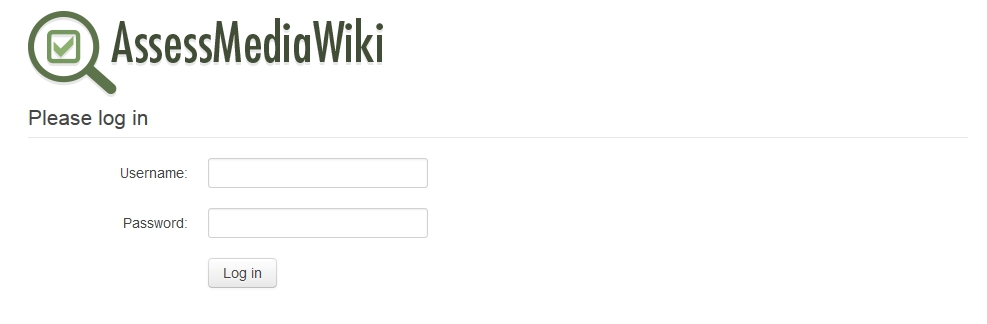
\includegraphics[width=0.9\textwidth]{sc_login.jpg}
	\caption{Pantalla de login.}
\end{figure}
\clearpage

Una vez iniciada sesión, si hay algún ejercicio de evaluación con preasignaciones realizadas, se mostrara a los alumnos un texto con un enlace a la edición que tienen que evaluar y varios campos con la información que deben rellenar.\\

\begin{figure}[h!]
	\centering
	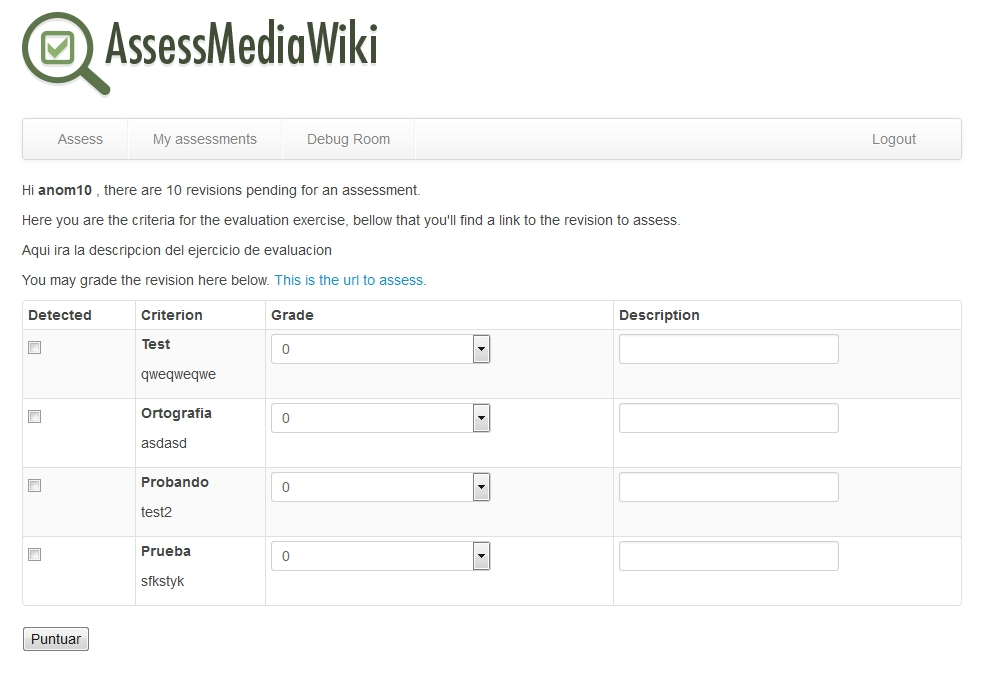
\includegraphics[width=0.9\textwidth]{sc_revision.jpg}
	\caption{Pantalla de inicio del usuario (sin la sala de debug, eso es debido a que el modo de desarrollo esta activado).}
\end{figure}
\clearpage

Por el contrario, si no tienen ninguna edición que evaluar se mostrara el siguiente mensaje:\\

\begin{figure}[h!]
	\centering
	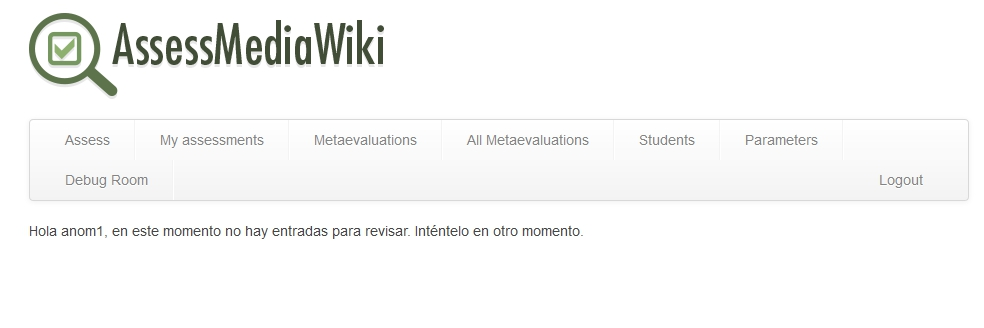
\includegraphics[width=0.9\textwidth]{sc_no_revision.jpg}
	\caption{Pantalla de usuario sin revisiones.}
\end{figure}
\clearpage

Si así lo deseamos podemos modificar los permisos del rol de alumnos o crear un rol especial para que algunos alumnos realicen metaevaluaciones sobre las evaluaciones realizadas.\\

su interfaz es similar a los anteriores, solo que en este caso no deberán evaluar varios criterios de la edición, sino que deberán evaluar en general la evaluación realizada sobre la edición\\

\begin{figure}[h!]
	\centering
	\includegraphics[width=0.9\textwidth]{sc_metaevaluar.jpg}
	\caption{Pantalla de metaevaluaciones.}
\end{figure}
\clearpage

Dependiendo del grado de responsabilidad y confianza que queramos darle al alumno podemos darle acceso a la lista de metaevaluaciones, si no esta lista sera solo accesible para el profesor / administrador, en la cual podrá ver todas las metaevaluaciones que han sido realizadas.\\

\begin{figure}[h!]
	\centering
	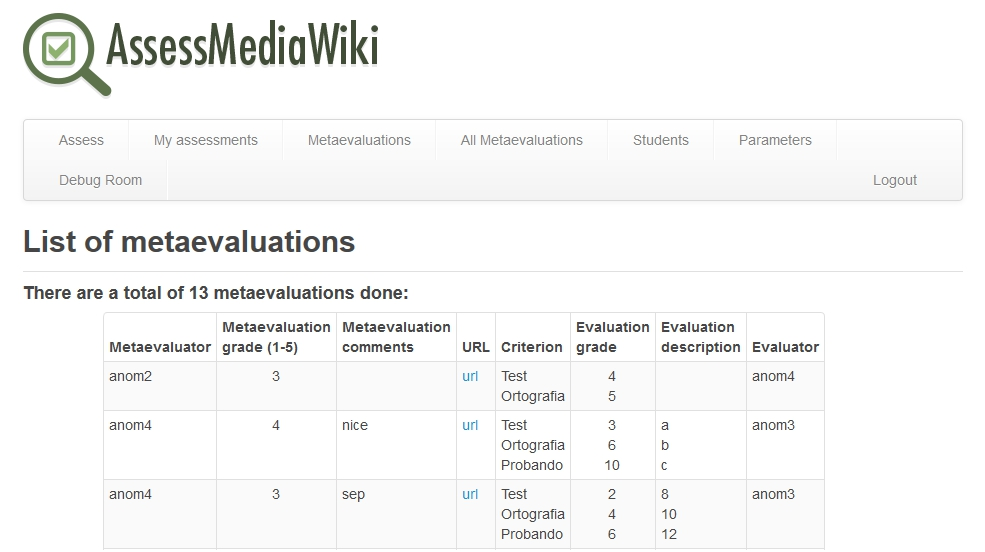
\includegraphics[width=0.9\textwidth]{sc_metaevaluar_lista.jpg}
	\caption{Pantalla de listado de metaevaluaciones.}
\end{figure}
\clearpage

En el apartado de la lista de estudiantes podemos ver el resumen de actividad de cada estudiante, ya sea por evaluaciones o metaevaluaciones realizadas y recibidas. También podemos generar un CSV (Coma Separated Values) con la información del alumno.\\

\begin{figure}[h!]
	\centering
	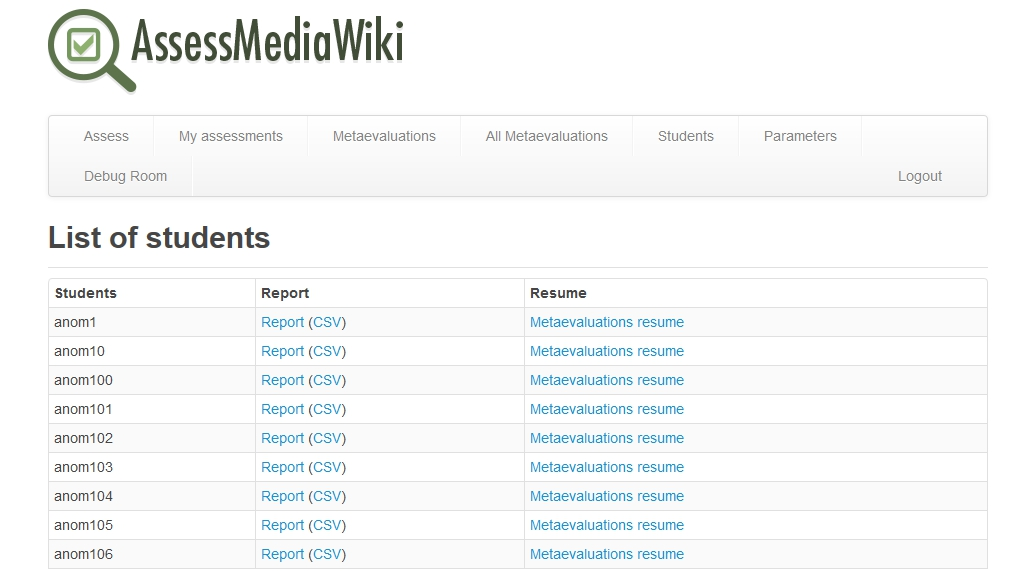
\includegraphics[width=0.9\textwidth]{sc_student_list.jpg}
	\caption{Pantalla de listado de alumnos.}
\end{figure}
\clearpage

A continuación tenemos los parámetros de AssessMediaWiki, aquí podemos definir las categorías a evaluar, si son genéricas o especificas y una lista de parámetros entre los que encontraremos los siguientes en esta nueva versión:\\

\begin{itemize}
	\item Ediciones evaluadas por alumno - numero de ediciones que serán evaluadas de cada alumno.
	\item Evaluaciones por edición - numero de evaluaciones que recibirá cada edición.
	\item Autoevaluaciones - para permitir que un alumno evalúe su propia edición si se diera el caso.
\end{itemize}

Para realizar cualquier cambio en alguno de estos parámetros solo tenemos que modificarlos y hacer clic en el botón "Modify parameters".\\

A través de este apartado de parámetros también podemos acceder a la administración de roles y ejercicios de evaluación, las cuales veremos a continuación.

\begin{figure}[h!]
	\centering
	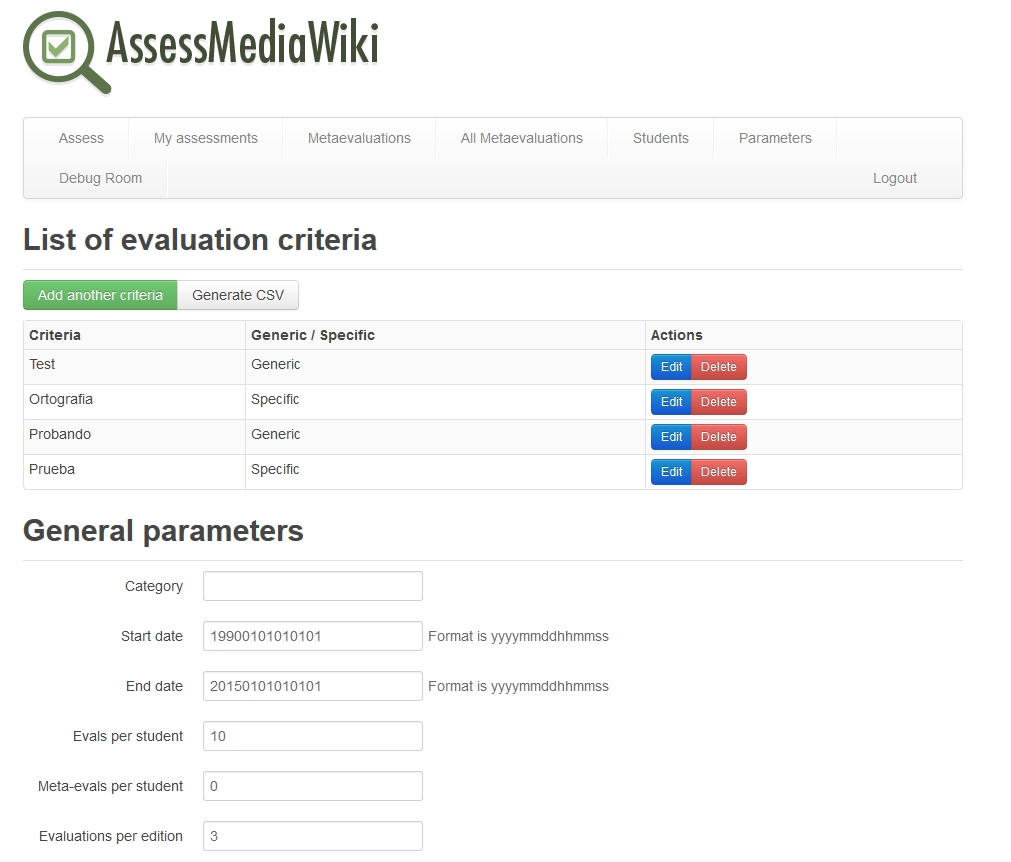
\includegraphics[width=0.9\textwidth]{sc_parametros1.jpg}
	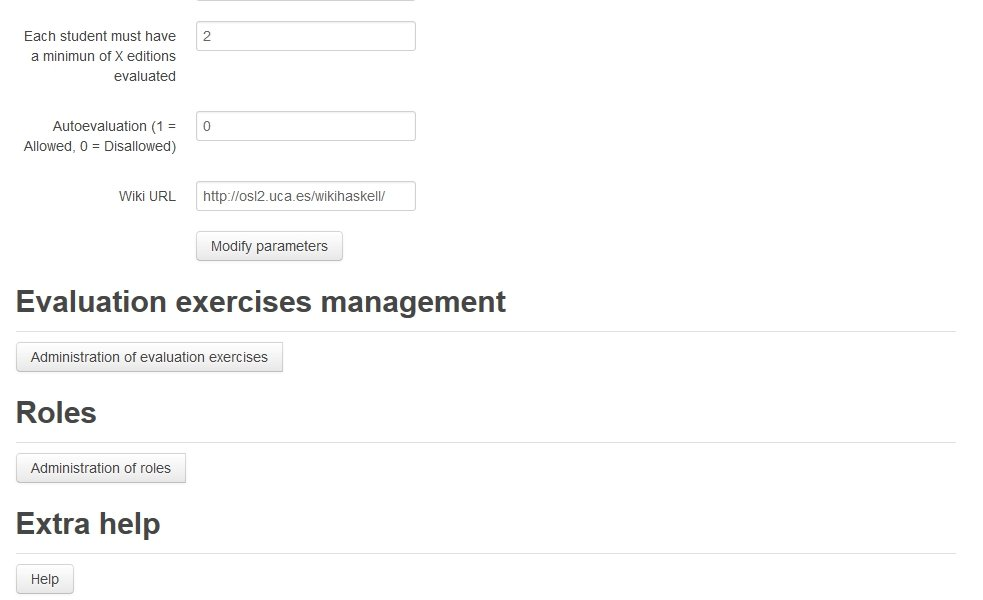
\includegraphics[width=0.9\textwidth]{sc_parametros2.jpg}
	\caption{Pantalla de parámetros.}
\end{figure}
\clearpage

En la pagina de administración de roles podremos editar los permisos de los roles existentes, crear roles, eliminarlos, asignarlos a un alumno y ver la lista de asignaciones realizadas.\\

Para modificar los permisos de un rol basta con seleccionar las casillas deseadas y hacer clic en el botón "Edit rol permissions" ubicado al final de la fila. \\

Para añadir un rol solo tenemos que escribir el nombre deseado del rol, seleccionar los permisos que le vamos a dar y hacer clic en el botón "Create rol".\\

Para eliminar un rol tan solo hay que seleccionarlo de la lista y hacer clic en "Delete rol", el propio sistema se encargaría de eliminar todas las asignaciones existentes si las hubiera.\\

Para asignarle un rol a un usuario tan solo debemos seleccionar el rol deseado y el usuario que recibirá dicho rol de las listas desplegables y presionar el botón "Assign rol". Cabe destacar que en la lista posterior a esta opción solo se mostraran aquellos usuarios con roles especiales, es decir, los que no sean estudiantes.\\

\begin{figure}[h!]
	\centering
	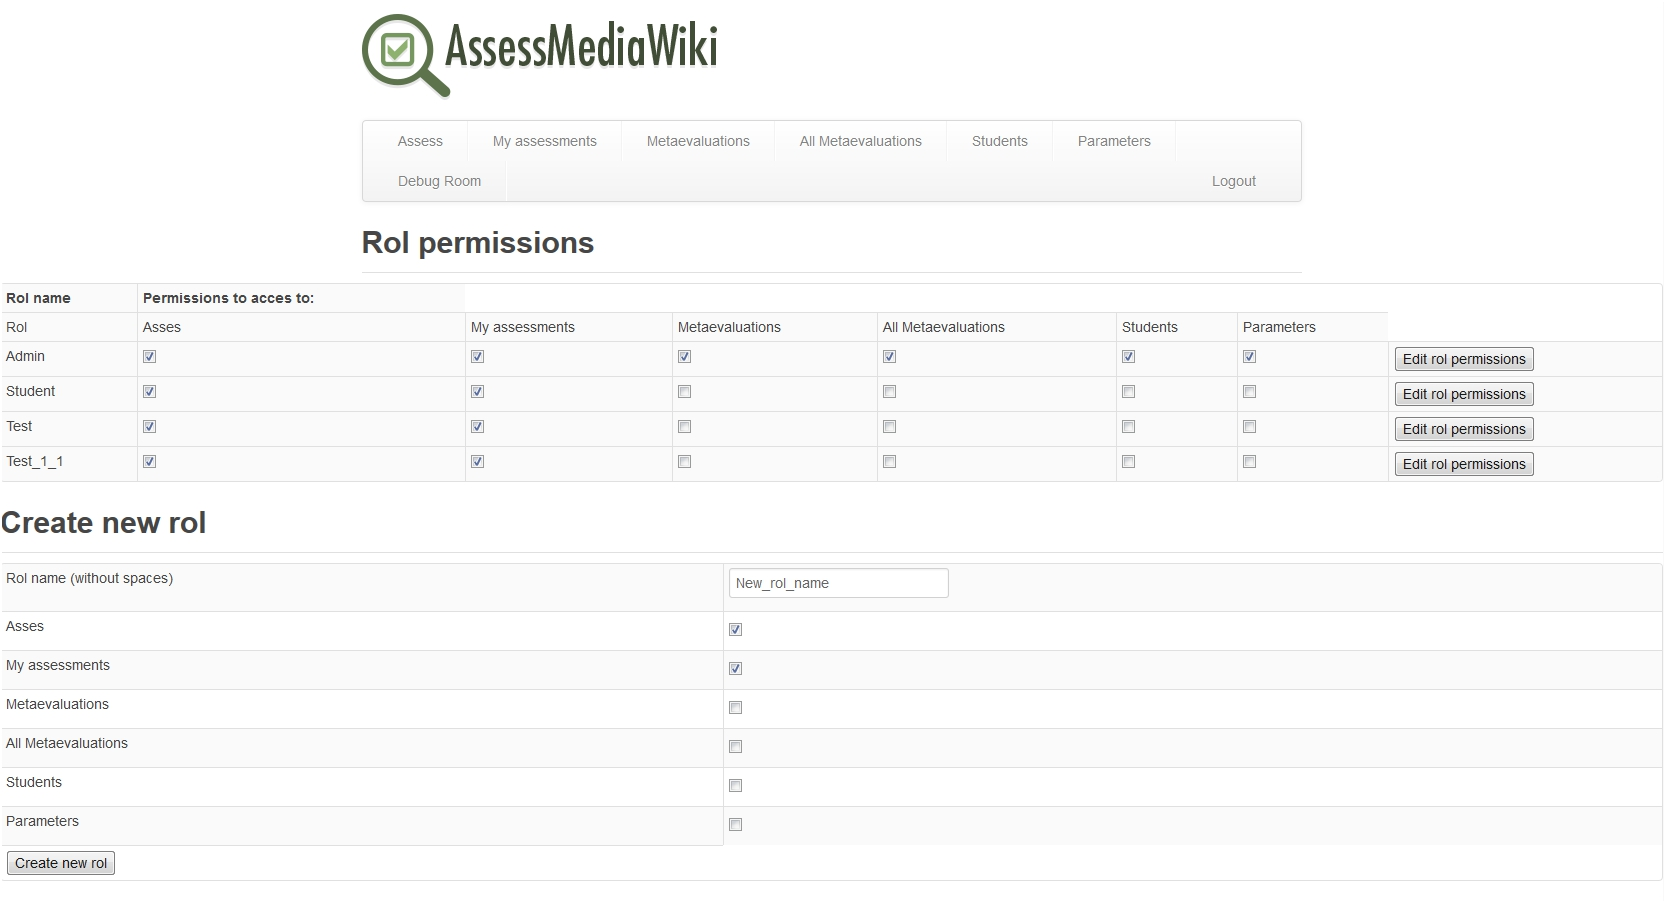
\includegraphics[width=0.9\textwidth]{sc_roles1.jpg}
	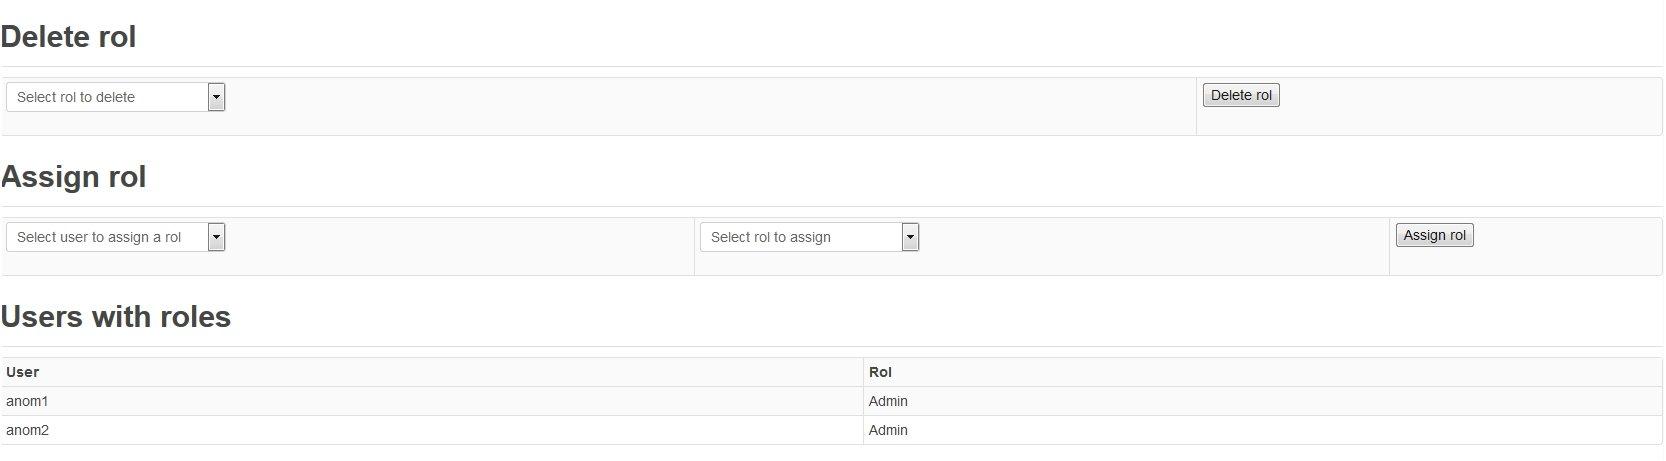
\includegraphics[width=0.9\textwidth]{sc_roles2.jpg}
	\caption{Pantalla de configuración de roles.}
\end{figure}
\clearpage

En la pagina de administración de ejercicios de evaluación podremos editar las propiedades de los ejercicios de evaluación existentes, crear ejercicios de evaluación, eliminarlos, editar las categorías a evaluar en cada uno de ellos y realizar y eliminar preasignaciones.\\

Para modificar los parámetros de un ejercicio de evaluación basta con modificar los datos de la fila correspondiente y hacer clic en el botón "Edit evaluación exercise" ubicado al final de la fila. \\

Para añadir un ejercicio de evaluación solo tenemos que escribir el nombre deseado del ejercicio de evaluación, introducir los datos deseados y hacer clic en el botón "Create new evaluation exercise".\\

Para eliminar un ejercicio de evaluación tan solo hay que seleccionarlo de la lista y hacer clic en "Delete evaluation exercise", pero a diferencia del caso de los roles el sistema mantendrá todas las evaluaciones referentes al ejercicio de evaluación, lo único que evitara es que modifiquemos los parámetros del mismo.\\

Para realizar o eliminar las preasignaciones de un ejercicio de evaluación tan solo debemos seleccionar el ejercicio de evaluación deseado en la lista desplegable y hacer clic en el botón "Make preasignations" o "Delete preasignations".\\ 

Cabe destacar que en las listas solo aparecerán los ejercicios de evaluación en los cuales no se hayan creado todavía las preasignaciones o se hayan realizado todas las evaluaciones para el caso de la creación de preasignaciones, y para el caso de eliminar las preasignaciones solo aparecerán aquellos ejercicios de evaluación para los que quede alguna preasignación pendiente de evaluar.\\

\begin{figure}[h!]
	\centering
	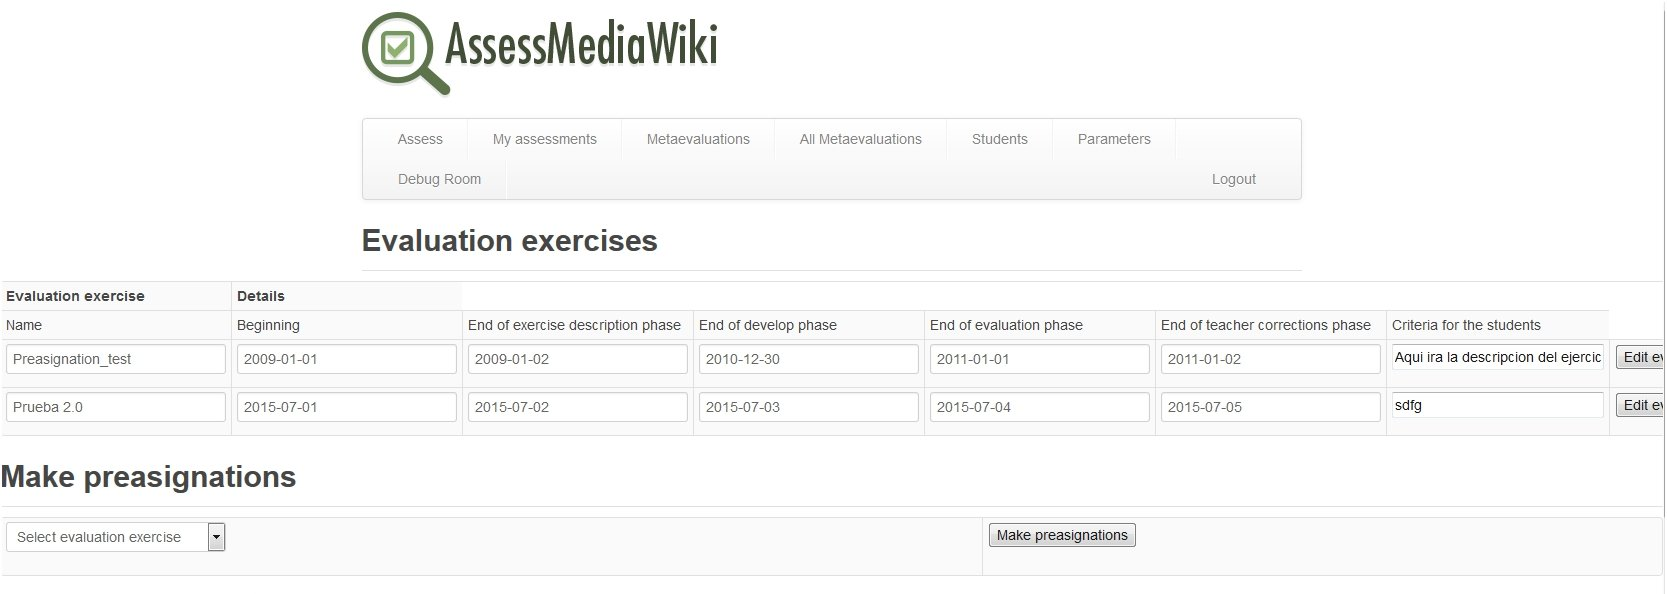
\includegraphics[width=0.9\textwidth]{sc_ee1.jpg}
	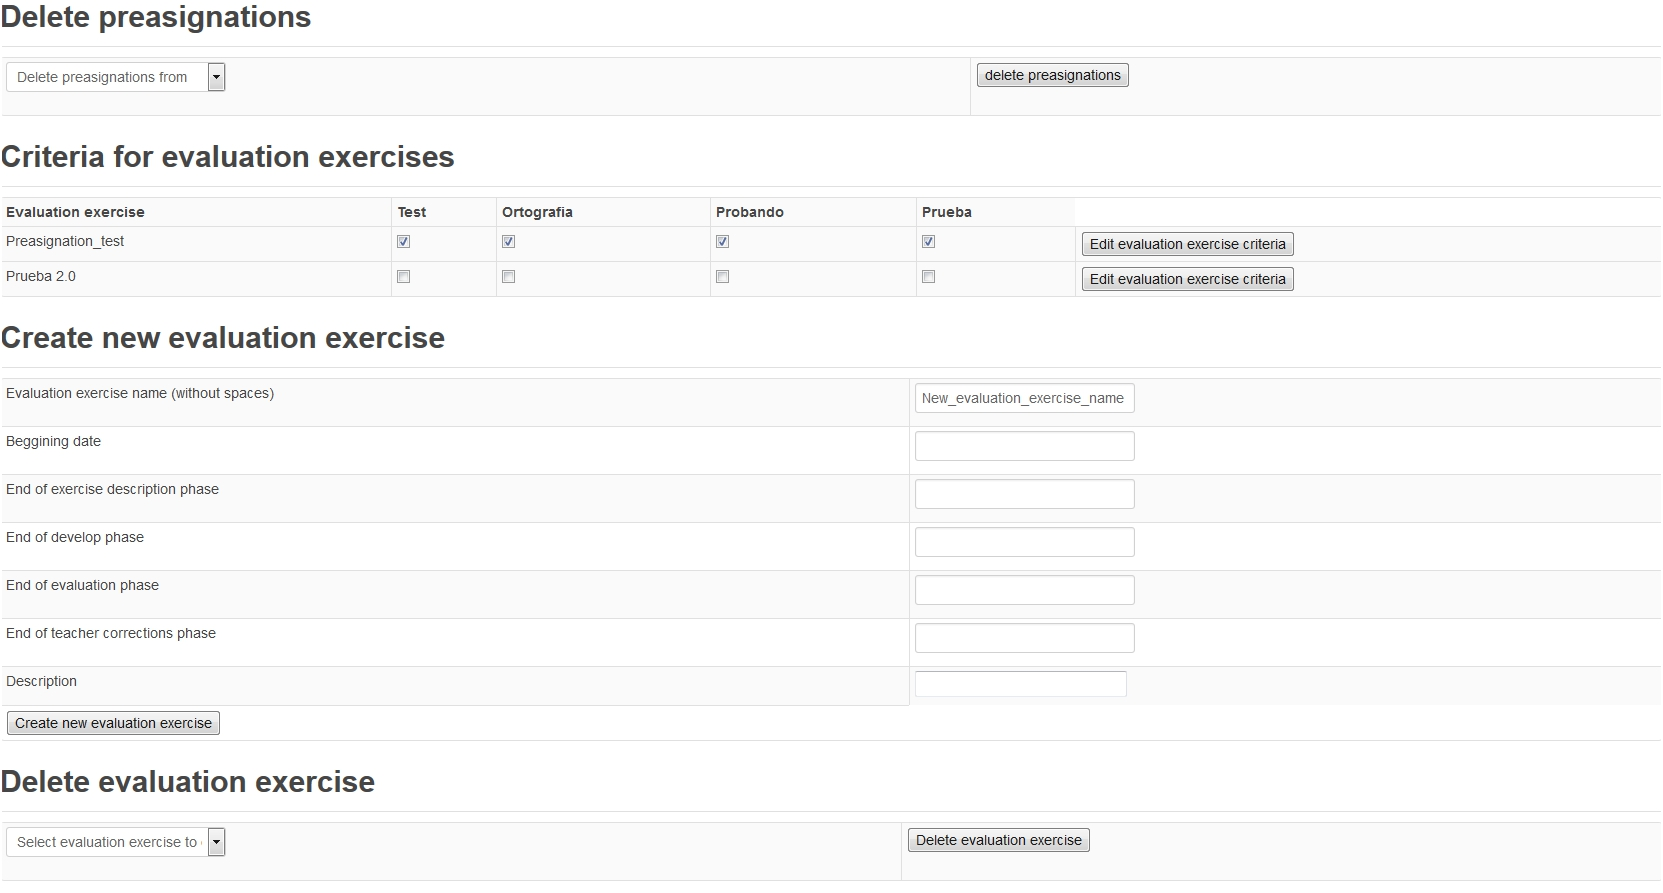
\includegraphics[width=0.9\textwidth]{sc_ee2.jpg}
	\caption{Pantalla de configuración de ejercicios de evaluación.}
\end{figure}
\clearpage

En caso de alguna duda o si fuese necesario un recordatorio, no será necesario consultar este manual una vez instalado el sistema, ya que el propio sistema al final la sección de parámetros tiene enlace a una sección de ayuda para el usuario, con información de las opciones configurables del sistema con las que el docente deberá trabajar.

\begin{figure}[h!]
	\centering
	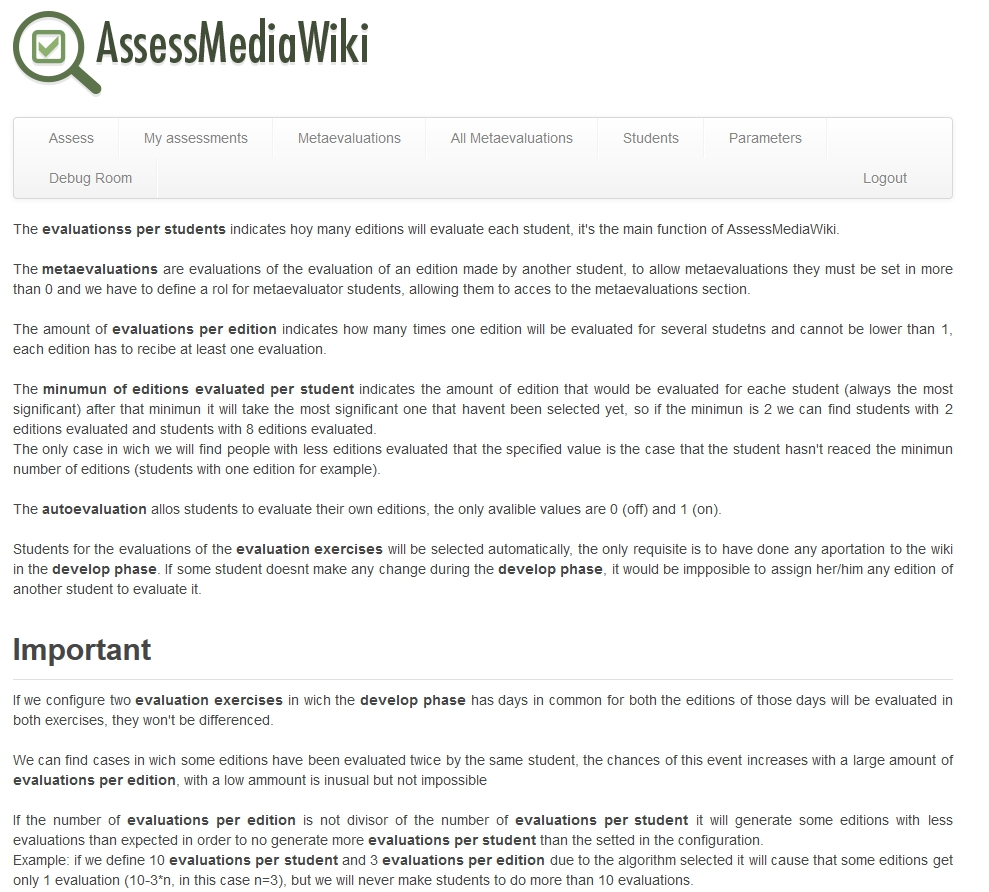
\includegraphics[width=0.9\textwidth]{sc_extra_help.jpg}
	\caption{Pantalla de ayuda extra.}
\end{figure}
\clearpage





